\documentclass{report}
\usepackage{hyperref}
\usepackage{tikz}
\title{Fake News Detection using NLP and Deep Learning}

\author{Research Team}
=======
\author{TODO: Author Name}

\date{\today}
\begin{document}
\maketitle
\begin{abstract}

This dissertation explores automatic detection of misinformation on the web.
We combine classical natural language processing with recent deep-learning
approaches to build a robust classifier for news articles.  The study describes
the dataset, modelling choices and the accompanying prototype application.
\end{abstract}
\tableofcontents

\chapter{Introduction}
The proliferation of unverified information on social media platforms has
raised significant concerns for policy makers and the general public.  This
chapter outlines the motivation for automated fake news detection and
summarises the objectives of the project, namely to evaluate a range of models
and deliver a lightweight web demonstration.

\chapter{Literature Review}
Research on misinformation spans linguistic features, network analysis and
machine learning.  Early approaches relied on handcrafted cues, whereas recent
work employs transformers such as BERT that learn context directly from data.
We review the strengths and limitations of these techniques and highlight open
challenges regarding bias and domain transfer.

\chapter{Methodology}
Our methodology begins with cleaning and normalising the news text before
extracting features.  Classical models use TF--IDF vectors with logistic
regression and tree ensembles, while the deep track experiments with recurrent
neural networks.  Training and validation procedures follow a stratified split
of the provided dataset.

\chapter{Experiments}
Experiments compare baseline classifiers against the proposed models.  We report
metrics such as accuracy and macro--F1 and include a brief error analysis.  The
results demonstrate that even simple models provide competitive performance on
this dataset, while deep networks require more resources but offer marginal
improvements.

\chapter{Discussion}
The discussion interprets the empirical findings and considers practical
implications.  We address limitations including dataset biases and the rapidly
changing nature of online discourse, arguing for continuous model updates and
human oversight.

\chapter{Conclusion}
We present a compact yet extensible framework for fake news detection that
integrates data processing, modelling and a demonstration interface.  Future
work will expand the training data and explore multilingual settings.


TODO: Abstract content.
\end{abstract}
\tableofcontents
\chapter{Introduction}
TODO: Introduction text.
\chapter{Literature Review}
TODO: Literature review text.
\chapter{Methodology}
The workflow for detecting fake news is illustrated in Figure~\ref{fig:pipeline}.

\begin{figure}[h]
    \centering
    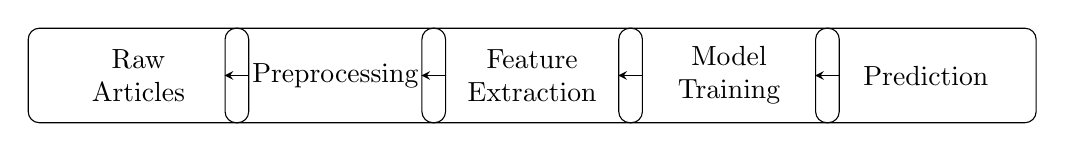
\begin{tikzpicture}[
        node distance=2.5cm,
        >=stealth,
        every node/.style={draw, rectangle, rounded corners, align=center, minimum width=2.8cm, minimum height=1.2cm}
    ]
        \node (data) {Raw\\Articles};
        \node (prep) [right of=data] {Preprocessing};
        \node (feat) [right of=prep] {Feature\\Extraction};
        \node (model) [right of=feat] {Model\\Training};
        \node (pred) [right of=model] {Prediction};

        \draw[->] (data) -- (prep);
        \draw[->] (prep) -- (feat);
        \draw[->] (feat) -- (model);
        \draw[->] (model) -- (pred);
    \end{tikzpicture}
    \caption{Processing pipeline used in this project.}
    \label{fig:pipeline}
\end{figure}

TODO: Methodology details.
\chapter{Experiments}
TODO: Experiments and results.
\chapter{Discussion}
TODO: Discussion.
\chapter{Conclusion}
TODO: Conclusion.

\bibliographystyle{plain}
\bibliography{refs}
\end{document}
